\documentclass[12pt,letterpaper]{article}
\usepackage{fullpage}
\usepackage[top=2cm, bottom=4cm, left=2.5cm, right=2.5cm]{geometry}
\usepackage{amsmath,amsthm,amsfonts,amssymb,amscd}
\usepackage{lastpage}
\usepackage{enumerate}
\usepackage{fancyhdr}
\usepackage{mathrsfs}
\usepackage{xcolor}
\usepackage{graphicx}
\usepackage{listings}
\usepackage{hyperref}
\usepackage{float}

\hypersetup{%
  colorlinks=true,
  linkcolor=blue,
  linkbordercolor={0 0 1}
}
 
\renewcommand\lstlistingname{Algorithm}
\renewcommand\lstlistlistingname{Algorithms}
\def\lstlistingautorefname{Alg.}

\lstdefinestyle{Python}{
    language        = Python,
    frame           = lines, 
    basicstyle      = \footnotesize,
    keywordstyle    = \color{blue},
    stringstyle     = \color{green},
    commentstyle    = \color{red}\ttfamily
}

\setlength{\parindent}{0.0in}
\setlength{\parskip}{0.05in}
\begin{document}

    \begin{enumerate}
        \item 
        \begin{enumerate}
            \item
                \begin{gather*}
                    \lim_{h \rightarrow 0} \frac{h-ln(1+h)}{h} = 0
                \end{gather*}
                Our third order taylor expansion for $ln(1+h)$ is: 
                \begin{gather*}
                    ln(1+h) \approx \frac{h^3}{3} -\frac{h^2}{2} + h
                \end{gather*}
                Therefore: 
                \begin{gather*}
                    \frac{h-(\frac{h^3}{3} -\frac{h^2}{2} + h)}{h} = \frac{h^2}{3} + \frac{h}{2}
                \end{gather*}
                So: 
                \begin{gather*}
                    \lim_{h \rightarrow 0} \frac{h-ln(1+h)}{h} = O(h^2 + h) = O(h^2)
                \end{gather*}
            \item 
                \begin{gather*}
                    \lim_{h \rightarrow 0} \frac{1}{1-h} = 1
                \end{gather*}
                Then,
                \begin{gather*}
                    |\alpha_{n} - \alpha| = \frac{1}{1-h} - 1 = \frac{1}{1-h} - \frac{1-h}{1-h} = \frac{h}{1-h}
                \end{gather*}
                and since 
                \begin{gather*}
                    |\frac{h}{1-h}| \leq |h|
                \end{gather*}
                for all positive integers h, we find that
                \begin{gather*}
                    \lim_{h \rightarrow 0} \frac{1}{1-h} = 1 + O(h)
                \end{gather*}
            \item 
            \begin{gather*}
                \lim_{h \rightarrow 0} \frac{hcos(h) - tan^{-1}(h)}{h} = 0
            \end{gather*}
            Our third order taylor expansion for $hcos(h) - tan^{-1}(h)$ is: 
            \begin{gather*}
                hcos(h) - tan^{-1}(h) \approx \frac{-h^3}{6}
            \end{gather*}
            Then: 
            \begin{gather*}
                \frac{\frac{-h^3}{6}}{h} = \frac{-h^2}{6}
            \end{gather*}
            So: 
            \begin{gather*}
                \lim_{h \rightarrow 0} \frac{hcos(h) - tan^{-1}(h)}{h} = O(h^2)
            \end{gather*}
        \end{enumerate}

        \item 
        \emph{Solution.} \\
        The geometric series for $|r| < 1$ sums to: 
        \begin{gather*}
            \sum^{\infty}_{k=0} r^k = \frac{1}{1-r}
        \end{gather*}

        If we move the starting $k$ and the $n$ by 2: 
        \begin{gather*}
            \lim_{n+2 \rightarrow \infty} \sum^{n+2}_{k=2} r^k = \lim_{n \rightarrow \infty} \frac{1-r^{n+3}}{1-r}
        \end{gather*}
        Therefore: 
        \begin{gather*}
            \frac{1-r^{n+3}}{1-r} = \frac{1}{1-r} - \frac{r^{n+3}}{1-r} = \frac{1}{1-r} - \frac{r^{n+3}}{r} = \frac{1}{1-r} - r^{n+2}
        \end{gather*}

        Thus: 
        \begin{gather*}
            \lim_{n+2 \rightarrow \infty} \sum^{n+2}_{k=2} r^k = \lim_{n \rightarrow \infty} \frac{1-r^{n+3}}{1-r} = \frac{1}{1-r} + O(r^{n+2})
        \end{gather*}
        So we see that we can generalize the convergence of $\sum^{\infty}_{k=i} r^k$ where 
        $i = 3, 4, 5, \dots$ as: 
        \begin{gather*}
            \lim_{n+i \rightarrow \infty} \sum^{n+i}_{k=i} r^k = \lim_{n \rightarrow \infty} \frac{1-r^{n+i}}{1-r} = \frac{1}{1-r} + O(r^{n+i})
        \end{gather*}

        \item 
        \begin{enumerate}
            \item 
            Multiplications: $\frac{n(n+1)}{2}$\\
            Additions: $\frac{n(n+1)}{2} - 1$
            \item 
            By taking the multiple $a_i$ out of every iteration of $i$, we can sum
            all of the $b_j$ and then multiply by $a_i$ to drastically reduce the 
            amount of multiplications: 
            \begin{gather*}
                \prod^{n}_{i = 1}a_{i}\sum^{i}_{j = 1}b_j
            \end{gather*}
            In this case, we still have $\frac{n(n+1)}{2}-1$ additions, but we only have 
            $n$ multiplications. 
        \end{enumerate}

        \item
        Looking at the estimations where $P1$ corresponds to $1 + 20x + 45x^2 + 120x^3 + 210 x^4 + 252x^5 + 210x^6+120x^7 + 45x^8 + 10x^9 + x^{10}$
        and $P2$ corresponds to $(x+1)^{10}$: \\
        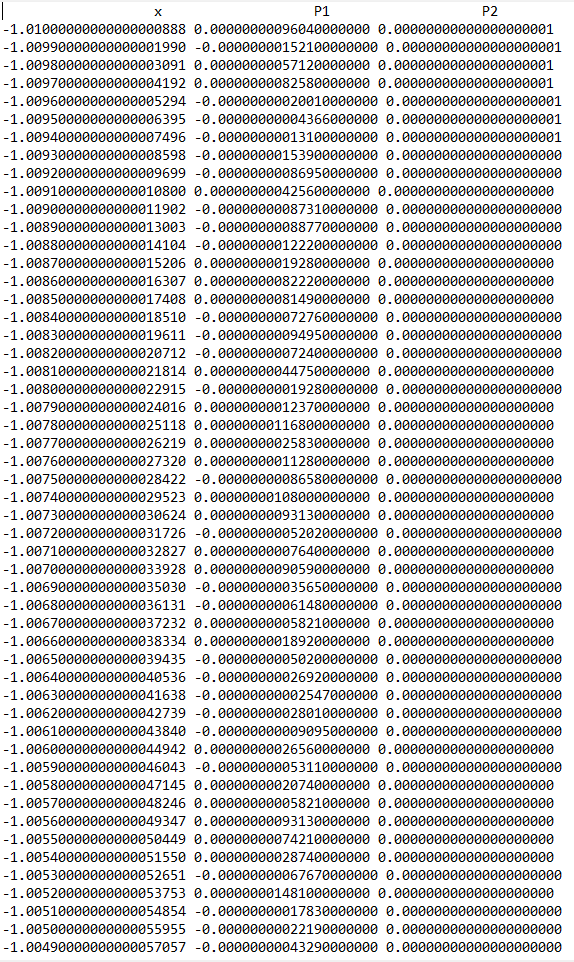
\includegraphics[scale = .8]{number4est.png}\\
        We see the $P2$ estimates are immediately zero, or extremely close to zero,
        while the $P1$ estimates float around the actual value of $P(-1)$. We also see this
        when we graph both equations: \\
        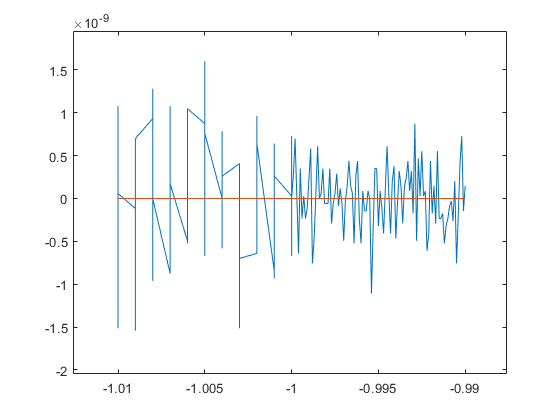
\includegraphics{number4graph.png}\\
        
    \end{enumerate}


\end{document}